\documentclass[a4paper, 12pt]{article}
\usepackage[a4paper,top=1.5cm, bottom=1.5cm, left=1cm, right=1cm]{geometry}

% Работа с русским языком
\usepackage[utf8]{inputenc}
\usepackage{mathtext}                % русские буквы в формулах
\usepackage[english, russian]{babel} % локализация и переносы

\usepackage{graphicx}   % Вставка изображений
\usepackage{float}      % "Плавающие" изображения3
\usepackage{wrapfig}    % Обтекание фигур (таблиц, картинок и прочего)
\usepackage{subfig}
\graphicspath{ {./images/} }

\usepackage{tabularx}
\usepackage{multirow}
\usepackage{amsmath}
\usepackage{amsfonts}
\usepackage{indentfirst}
\usepackage{longtable}
\graphicspath{{pictures/}}
\usepackage{natbib}
\usepackage{bm}

%%% Колонтитулы
\usepackage{titleps}
\newpagestyle{main}{
	\setheadrule{0.4pt}
	\sethead{Исследование эффекта Комптона}{}{}
	\setfootrule{0.4pt}                       
	\setfoot{ФРКТ МФТИ, 2024}{}{\thepage} 
}
\pagestyle{main}  

\begin{document}
    \begin{titlepage}
	\begin{center}
            {\large МОСКОВСКИЙ ФИЗИКО-ТЕХНИЧЕСКИЙ ИНСТИТУТ (НАЦИОНАЛЬНЫЙ ИССЛЕДОВАТЕЛЬСКИЙ УНИВЕРСИТЕТ)}
	\end{center}
 
	\begin{center}
		{\large Физтех-школа радиотехники и компьютерных технологий}
	\end{center}
	
	\vspace{8cm}
	{\LARGE
		\begin{center}
                {\bf Отчёт о выполнении лабораторной работы 1.2}\\
                Исследование эффекта Комптона
		\end{center}
	}
	\vspace{5cm}
	\begin{flushright}
		{\Large Авторы: \\ 
        Тихонов Дмитрий Романович, \\ студент группы Б01-206а \\
        Павловский Кирилл Михайлович, \\ студент группы Б01-206а}
	\end{flushright}
	\vspace{4cm}
	\begin{center}
		\Large Долгопрудный, 2024
	\end{center}
    \end{titlepage}


    \section{Введение}

    \noindent \textbf{Цель работы:} исследовать энергетический спектр $\gamma$-квантов, рассеянных на графите и определить их энергию в зависимости от угла рассеяния, а также энергию покоя частиц, на которых происходит комптоновское рассеяние \\

    \noindent \textbf{В работе используются:} источник излучения, графитовая мишень, сцинтилляционный спектрометр, фотоэлектронный умножитель (ФЭУ), ЭВМ
    
    \section{Теоретические сведения}
    
    Эффект Комптона -- увеличение длины волны рассеянного излучения по сравнению с падающим в результате упругого соударения двух частиц: $\gamma$-кванта и свободного электрона.

     \begin{figure}[H]
        \centering
        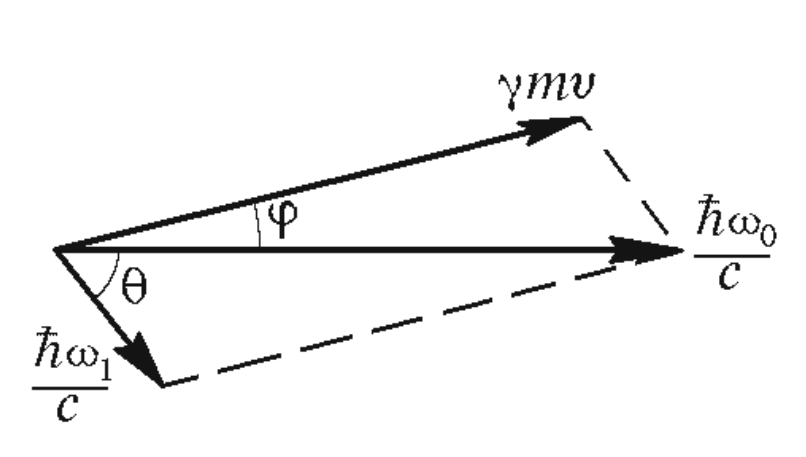
\includegraphics[scale = 0.25]{images/vector_diagram.png}
        \caption{Векторная диаграмма рассеяния $\gamma$-кванта на электроне}
        \label{diagram}
	\end{figure}

    Запишем для рассматриваемого процесса (рис. \ref{diagram}) ЗСЭ и ЗСИ:
	\begin{equation*}
	    \begin{gathered}
    	    m c^2 + \hbar \omega_0 = \gamma m c^2 +\hbar \omega_1,\\
    		\dfrac{\hbar \omega_0}{c} = \gamma m v \cos \phi + \dfrac{\hbar \omega_1}{c} \cos \theta,\\
    		\gamma m v \sin \phi = \dfrac{\hbar \omega_0}{c} \sin \theta.
	    \end{gathered}
	\end{equation*}

	Решая совместно эти уравнения и переходя от частот $ \omega_0 $ и $ \omega_1 $ к	длинам волн $ \lambda_0 $ и $ \lambda_1 $, нетрудно получить, что изменение длины волны	рассеянного излучения равно
 
	\begin{equation}
    \label{eq:main}
		\lambda_1 - \lambda_0 = \dfrac{h}{m c}\left(1- \cos \theta \right) = \Lambda_\text{к} \left(1- \cos \theta \right),
	\end{equation}
	где $$ \Lambda_\text{к} = \dfrac{h}{m c} = 2.42\cdot 10^{-10}\; см $$ называется комптоновской длиной волны электрона.
	
	В приведенном выводе электрон в атоме считается свободным. Для $\gamma$-квантов с энергией в несколько десятков, а тем более сотен кэВ,	связь электронов в атоме, действительно,	мало существенна, так как энергия их связи в легких атомах не превосходит нескольких кэВ, а для большинства электронов еще меньше.
	
    Применительно к условиям нашей работы формулу \eqref{eq:main} следует	преобразовать от длин волн к энергии $\gamma$-квантов
    
	\begin{equation}
    \label{eq:main_norm}
		\dfrac{1}{\varepsilon(\theta)} - \dfrac{1}{\varepsilon_0} = 1- \cos(\theta),
	\end{equation}
 
	где $ \varepsilon_0 = E_0/(m c^2) $  -- нормированная энергия $\gamma$-квантов, падающих на рассеиватель, $ \varepsilon(\theta) $ — выраженная в тех же единицах энергия квантов, испытавших комптоновское рассеяние на угол $\theta$, $ m $ -- масса электрона.

    \newpage
    
    \section{Методика измерений и экспериментальная установка}
	
	Схема экспериментальной установки отображена на рис. \ref{installation}.	
 
	\begin{figure}[H]
		\centering
		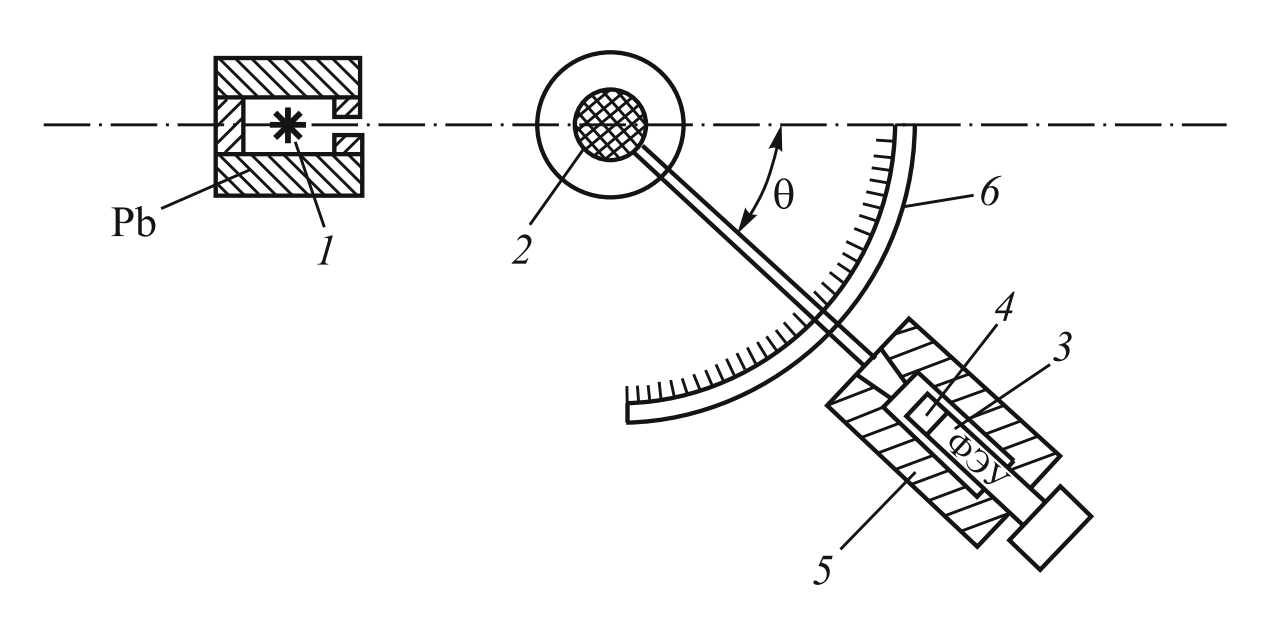
\includegraphics[width=0.7\linewidth]{images/installation.png}
		\caption{Схема экспериментальной установки}
		\label{installation}
	\end{figure}
 
	Сформированный коллиматором узкий пучок $\gamma$-квантов попадает на графитовую мишень. Кванты, испытавшие комптоновское рассеяние в мишени, регистрируются сцинтилляционным счетчиком, состоящим из сцинтиллятора и ФЭУ, работающего от высоковольтного источника напряжения. Сигнал, генерируемый ФЭУ, обрабатывается АЦП компьютера, и соответствующий график выводится на экран.

    \newpage
	
    \section{Результаты измерений и обработка данных}

    Заменим в формуле (\ref{eq:main_norm}) энергию квантов, испытавших комптоновское рассеяние на угол $\theta$, номером канала $N(\theta)$, соответствующего вершине фотопика при указанном угле $\theta$. Обозначая буквой $A$ неизвестный коэффициент пропорциональности между $\varepsilon(\theta)$ и $N(\theta)$, найдём:
    
	\begin{equation}
        \label{eq:main_final}
		\dfrac{1}{N(\theta)} - \dfrac{1}{N(0)} = A (1- \cos{\theta}).
	\end{equation}
 
	Представим экспериментальные результаты (табл. \ref{table}) в виде графика на рис. \ref{graph}, откладывая по оси абсцисс $1-\cos(\theta) $, а по оси ординат -- $ {1}/{N(\theta)} $.
	\begin{figure}[H]
		\centering
		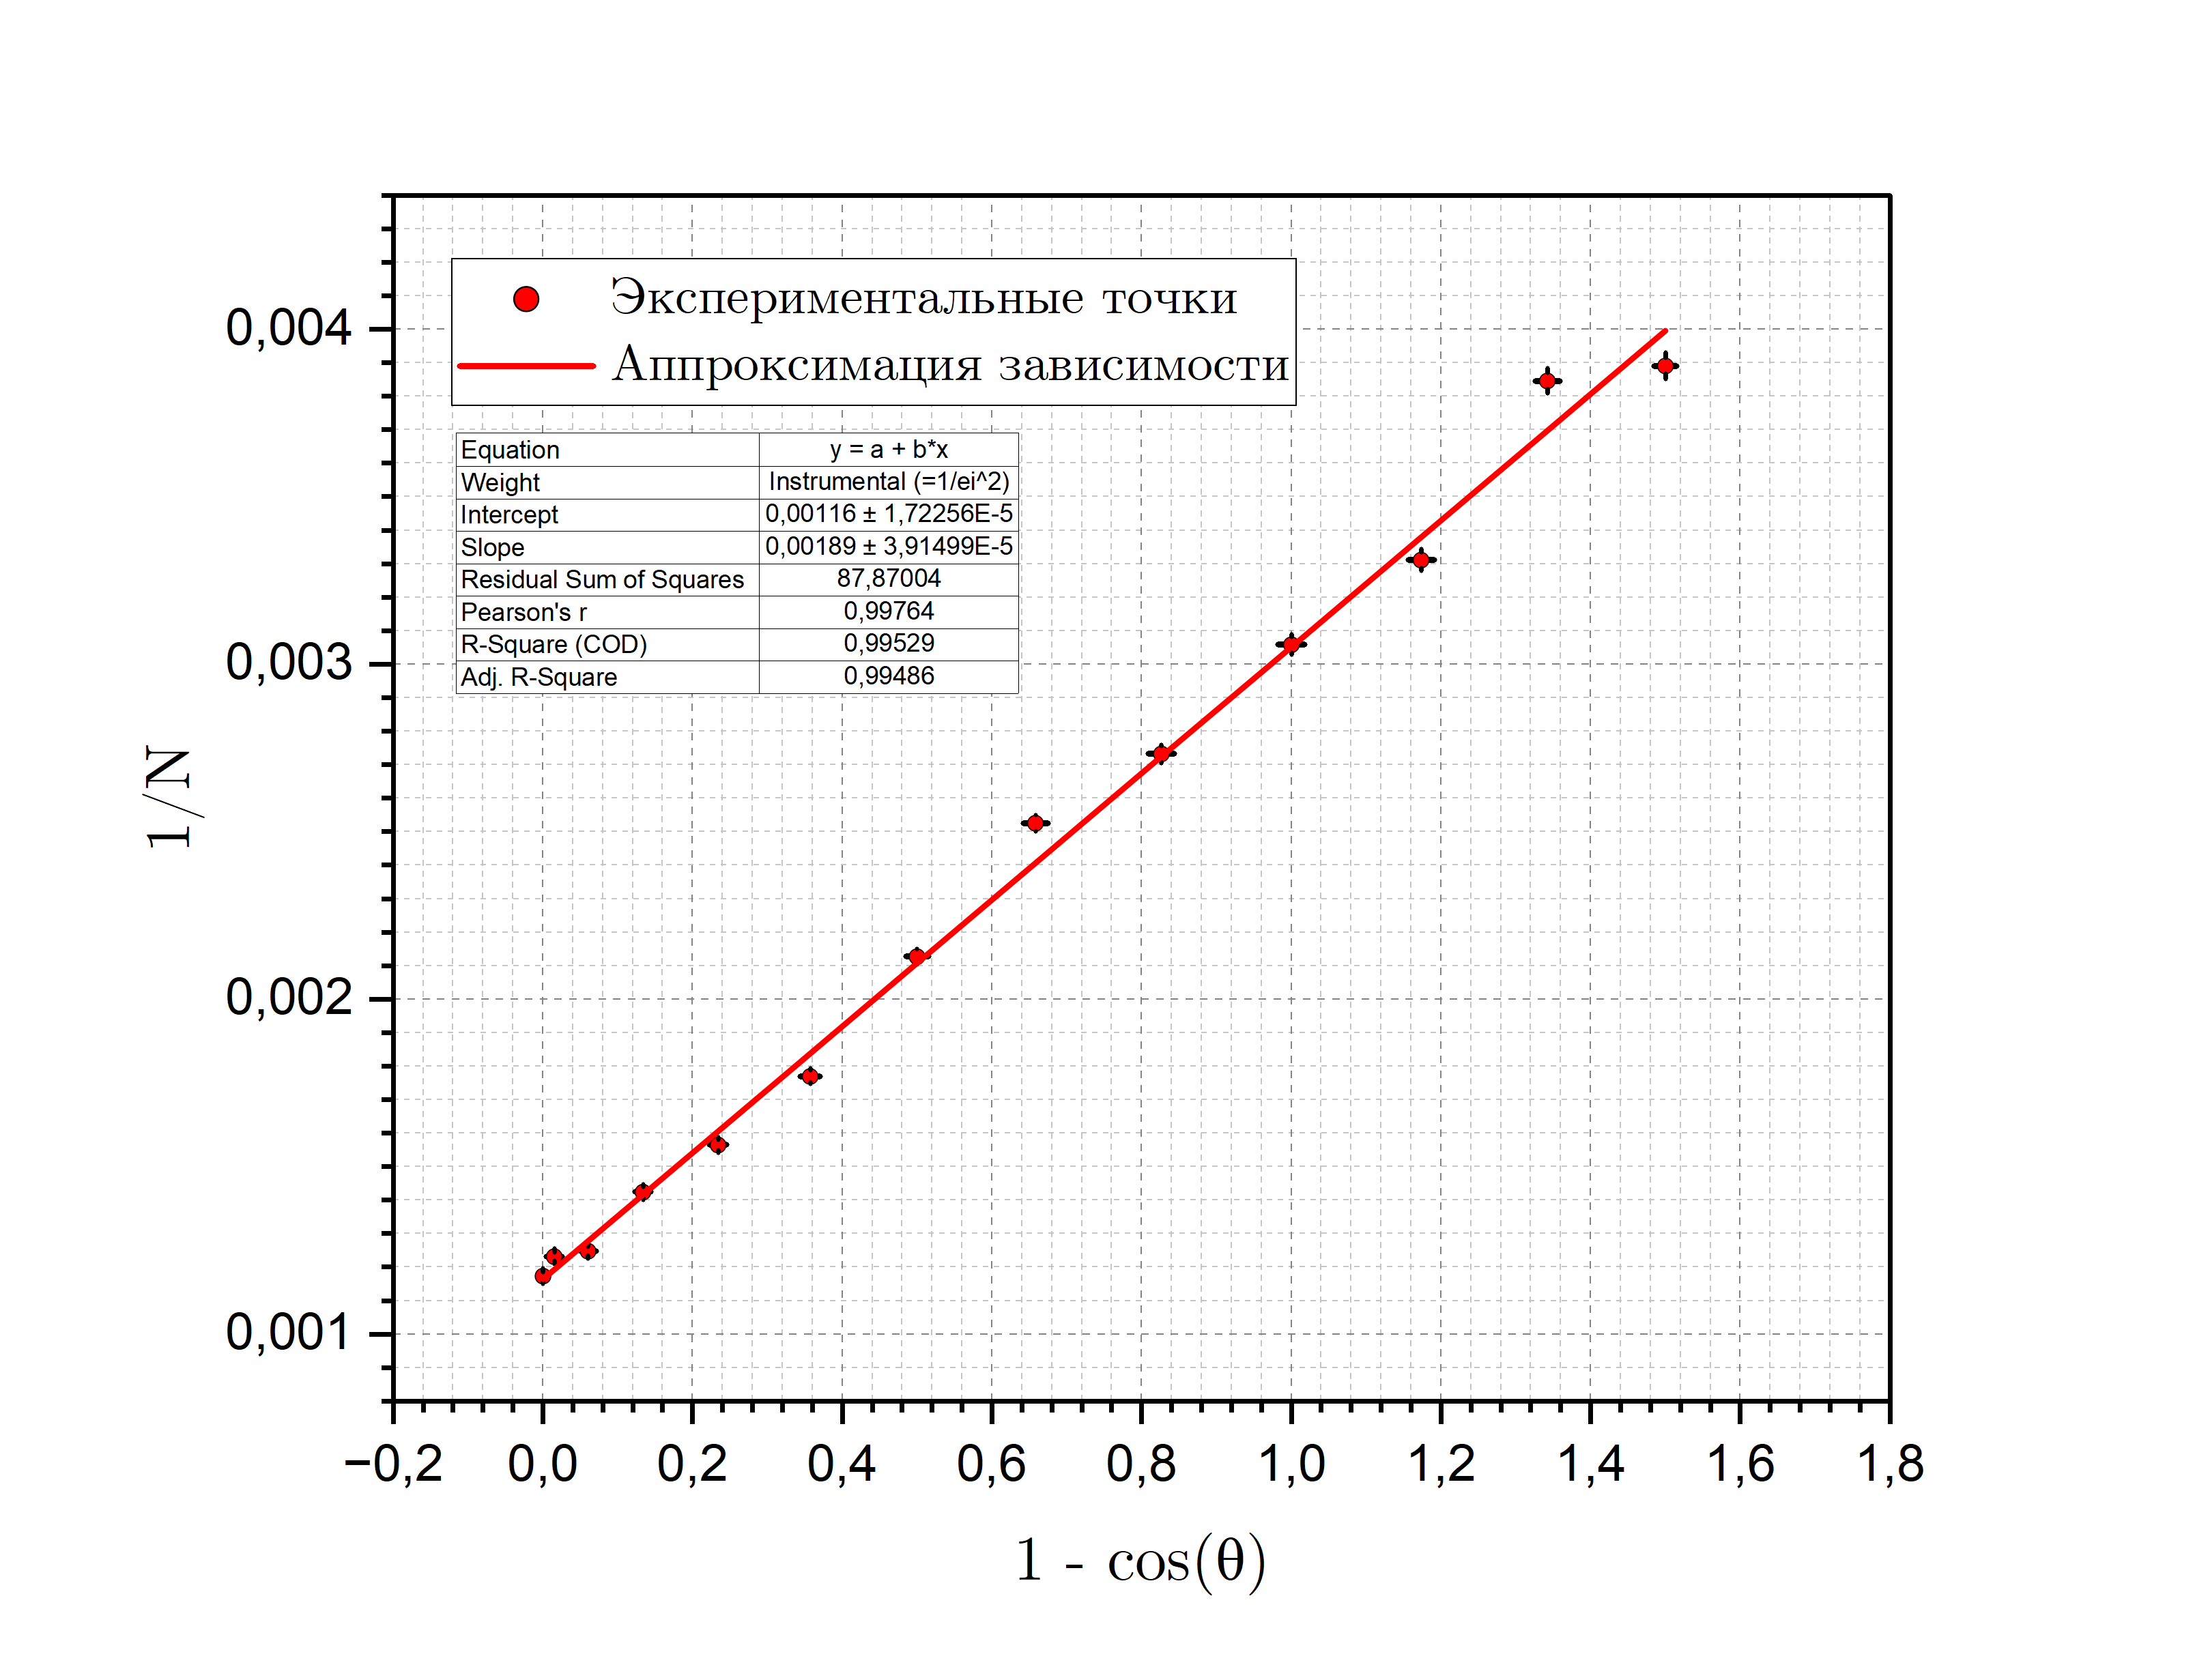
\includegraphics[width = 14 cm]{images/graph.png}
		\caption{График зависимости $\frac{1}{N} = f(1-\cos{\theta}$}
		\label{graph}
	\end{figure}
 
	По пересечению графика с осью ординат определим $N(0)$:
	$$N(0) = \left( 860 \pm 15 \right),$$ 
    где $N(0) = \frac{1}{b}$, а $\varepsilon_{N(0)} = \frac{\sigma_b}{b}$.
	
	По пересечению графика с прямой $\cos \theta = 0$ определим $N(90)$:
	$$N(90) = \left( 330 \pm 5 \right),$$
	где $N(90) = \frac{1}{b + a}$, а $\sigma_{N(90)} = \frac{1}{(a + b)^2}\sqrt{\sigma_b^2 + \sigma_a^2}$
	
	Определим энергию покоя электронов, на которых происходили рассеяния гамма-квантов:
	$$
	mc^2 = E_\gamma \frac{N(90)}{N(0) - N(90)} = \left( 410 \pm 15 \right) \text{ кэВ},
	$$
	где $E_\gamma = (662 \pm 1) кэВ$ -- энергия гамма-лучей, испускаемых источником. 
 
    Оценим погрешность определения $mc^2$:\\
	$$\sigma_{mc^2} = \sqrt{\left(\frac{N(90)}{N(0) - N(90)} \sigma_{E_\gamma} \right)^2 + \left(\frac{N(90) E_\gamma}{(N(0) - N(90))^2} \sigma_{N(0)}\right)^2 + \left(E_\gamma \frac{N(0)}{(N(0) - N(90))^2}\sigma_{N(90)}\right)^2}$$

    \section{Заключение}

    По результатам работы, исследовали эффект Комптона на графитовом образце с помощью сцинтилляционного спектрометра. Выяснили зависимость  энергии рассеянного $\gamma$-кванта от угла рассеяния, а также определили по порядку величины энергию покоя электрона.

    \newpage

    \section*{Приложение}

    \begin{table}[H]
        \centering
        \begin{tabular}{|c|c|c|c|}
        \hline
         $\theta, ^\circ$ & $\Delta \theta, ^\circ$ &  $N$, кан. & $\Delta N$, кан. \\ \hline
        0                     & \multirow{13}{*}{1} & 852                      & 8,52   \\ \cline{1-1} \cline{3-4} 
        10                    &                     & 812                      & 8,12   \\ \cline{1-1} \cline{3-4} 
        20                    &                     & 801                      & 8,01   \\ \cline{1-1} \cline{3-4} 
        30                    &                     & 702                      & 7,02   \\ \cline{1-1} \cline{3-4} 
        40                    &                     & 639                      & 6,39   \\ \cline{1-1} \cline{3-4} 
        50                    &                     & 565                      & 5,65   \\ \cline{1-1} \cline{3-4} 
        60                    &                     & 470                      & 4,70   \\ \cline{1-1} \cline{3-4} 
        70                    &                     & 396                      & 3,96   \\ \cline{1-1} \cline{3-4} 
        80                    &                     & 366                      & 3,66   \\ \cline{1-1} \cline{3-4} 
        90                    &                     & 327                      & 3,27   \\ \cline{1-1} \cline{3-4} 
        100                   &                     & 302                      & 3,02   \\ \cline{1-1} \cline{3-4} 
        110                   &                     & 260                      & 2,60   \\ \cline{1-1} \cline{3-4} 
        120                   &                     & 257                      & 2,57   \\ \hline
        \end{tabular}

        \caption{Экспериментальные данные}
        \label{table}
    \end{table}

\end{document}